We explore applications of {\sc Ludus} to problems that game designers commonly face.

\subsection{Group Versus Round-Robin Tournament}

% Maybe explain the group tournament in more detail
The first experiment %we ran
investigates the efficacy of our approximation algorithm in Section~\ref{sec:tourney}. To do this, we compare the win rates %identical decks in
of a complete round-robin tournament (every combination of decks played) with the distribution of win rates over a 16-fold tournament of %conducted by
randomly partitioned decks into groups of various sizes, playing every combination of the decks within those groups.

\begin{figure}[t]
	\centering
	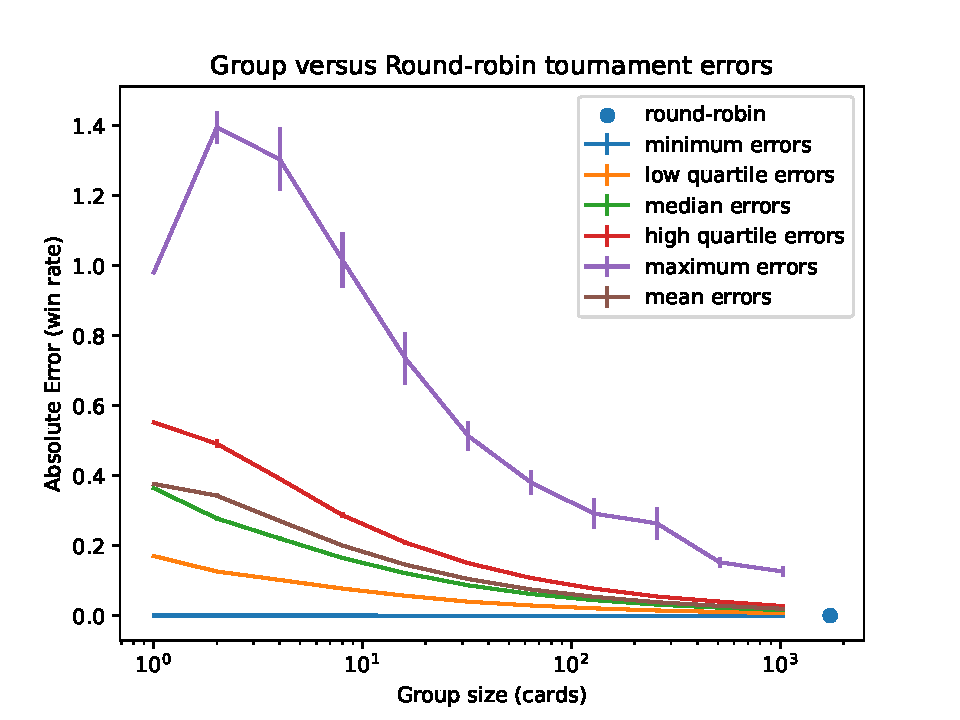
\includegraphics[width=0.9\columnwidth]{group_vs_rr_fig}
	\caption{Absolute value of the difference in win rate between a \textit{group tournament} of varying size and a full round-robin tournament of 1,728 possible decks. %, along with error bars.
	}
	\label{fig:group_vs_rr}
\end{figure}

%% Table

Figure~\ref{fig:group_vs_rr} compares the win rates of each deck in the group tournament versus the round-robin tournament, and we can see that at a group size of 256, the mean error becomes negligible (about 0.0382). We use this group size in the other experiments rather than a round-robin of all 1,728 decks.

% Another table

 \subsection{Optimizing Cards without Special Mechanics}

The next experiment optimizes a set of four `vanilla' cards with no extra mechanics. We expected that the `optimal' solution in terms of the standard deviation metric would have four identical cards because the interchangeable cards should have zero standard deviation in the win rate. Due to the limited number of generations in our genetic algorithm, we recognized that there was no guarantee it would find this solution. From a game design perspective, a less-optimal solution seems more interesting in this case as a game with only a single card is obviously uninteresting. We wanted to see what `almost-optimal' solutions appear for this setup. This observation also illustrates a case where the standard deviation metric fails to fully capture the qualities we wish to optimize in our game.

The results of this experiment illustrate a different failure case of our standard deviation metric that we did not predict. The genetic algorithm quickly found the solution (5/3), (5/4), (8/3), (8/1) where ($a$,$b$) indicates a card with $a$ attack and $b$ health points. This solution had the optimal zero standard deviation---why? Any pairing of these cards will result in both cards killing each other simultaneously. Thus, every game ends after one round of combat phases in a tie, and there is no variance in win rates amongst the decks. 

 \subsection{Optimizing Only Special Mechanics}

The third experiment optimizes only the special mechanic parameters of twelve cards. We assigned each card an intuitive value for its attack and health, which a game designer might do for initial context. {\sc Ludus} then optimized the parameters for the special mechanics of these partially-designed cards. We were interested to see how it %feasible it is to optimize the game with
optimized under these constraints and how impactful the special mechanics would be for the overall balance. %of the game.
Table~\ref{tab:special_cards} describes the cards used in this experiment. The optimizer improved the win rate standard deviation from 0.0751 to 0.0589. 

\begin{table*}[t]
\centering
\caption{Variable and Fixed Parameters for the \textit{Optimize Special Mechanics} Experiment}
\label{tab:special_cards}
\begin{tabular}{||c c c c c||} 
 \hline
 Card & Attack & Health & Special Parameter (see Section~\ref{sec:ab-game-def}) &  Optimized Special parameter\\ [0.5ex] 
 \hline\hline
 Explode On Death & 2 & 1 & Explosion Damage & 1\\ 
 \hline
 Friendly Vampire & 1 & 3 & Heal Amount & 3 \\
 \hline
 Grow On Damage & 0 & 5 & Attack Growth Per Hit & 4 \\
 \hline
 Heal On Death & 1 & 2 & Explosion Health & 3 \\
 \hline
 Health Donor & 1 & 4 & Heal Donation Percent & 3 \\
 \hline
 Ignore First Damage & 2 & 1 & Armor Points & 1 \\
 \hline
 Morph Attack & 0 & 3 & Morphing Enemies & N/A \\
 \hline
 Pain Splitter & 2 & 2 & Damage Split Percent & 7 \\
 \hline
 Rampage & 0 & 4 & Middle Age & 8 \\
 \hline
 Survivalist & 2 & 2 & Survivalist & N/A \\
 \hline
 Threshold & 2 & 2 & Target Age & 5 \\
 \hline
 Time Bomb & 1 & 8 & Detonation Time & 7 \\ 
 \hline
\end{tabular}
\end{table*}

\subsection{Optimizing All Parameters} \label{sec:first_set}

After fixing the attack and health to focus solely on the special mechanics, the next experiment tunes the attack, health, and special mechanics all at once. To reduce the huge dimensionality of this experiment, we selected only five of the twelve cards to optimize. They are listed in Table~\ref{tab:first_set}.

% First Set
\begin{table*}[t]
\centering
\caption{List of Cards in the First Set and Their Optimized Solution}
\label{tab:first_set}
\begin{tabular}{||c c c c||} 
 \hline
 Card & Optimized Attack & Optimized Health & Optimized Special Mechanic (see Section~\ref{sec:ab-game-def})\\ [0.5ex]
 \hline\hline
 Survivalist & 9 & 1 & N/A \\
 \hline
 Morph Attack & 5 & 5 & N/A \\
 \hline
 Ignore First Damage & 6 & 8 & 1 \\
 \hline
 Explode On Death & 4 & 1 & 3 \\ 
 \hline
 Vanilla & 7 & 2 & N/A \\
 \hline
\end{tabular}
\end{table*}

The optimizer improved the win rate standard deviation from 0.0704 to 0.0584. This minimum is approximately the same as the one achieved in the previous experiment, modifying only the values of the special mechanics. One important observation we made is that the optimizer was still making good progress in the final generations of both our experiments. This indicates that these might not be minima, %are not global, but that with
and compute time for additional generations could continue to improve the card designs.

\subsection{Optimizing After a Set Rotation}

Another common scenario designers of deck-building games encounter is releasing a new set %or batch
of cards that maintain the compatibility, fairness, and competitiveness with the previously released cards. %These expansions add new content to the game to keep it fresh.
To apply {\sc Ludus} to this problem, we took the set of five cards from Section~\ref{sec:first_set} with their optimized solution as %This represents
the first set of cards released. Next, we selected five additional cards, described in table Table~\ref{tab:second_set}, and optimized them alongside %, while keeping the values from
the first set fixed at the solution found previously---this is ten cards with variable parameters for only the second set of cards. 

% Compare this to the solution found by treating all 10 cards as one set

% Second Set
\begin{table*}[t]
\centering
\caption{List of Cards in the Second Set and Their Optimized Solution}
\label{tab:second_set}
\begin{tabular}{||c c c c||} 
 \hline
 Card & Optimized Attack & Optimized Health & Optimized Special Mechanic (see Section~\ref{sec:ab-game-def})\\ [0.5ex]
 \hline\hline
 Friendly Vampire & 7 & 7 & 8 \\
 \hline
 Grow On Damage & 2 & 6 & 9 \\
 \hline
 Heal On Death & 3 & 9 & 1 \\
 \hline
 Rampage & 6 & 7 & 5 \\ 
 \hline
 Vanilla & 7 & 6 & N/A \\
 \hline
\end{tabular}
\end{table*}

The optimizer improved the win rate standard deviation from 0.0591 to 0.0541. This is a comparatively smaller improvement than the previous experiments, %however,
but the initial state was already in much better condition than any of the previous experiments. This is interesting because it could indicate that adding new cards to an already well-balanced set may not disturb the balance as much as one might expect. 


% \subsubsection{Optimizing an exhaustive round-robin tournament}
